\subsection{Initial independent tests of the integrated calculation}
The initial comparison uses eight physical profiles that did not select the
weights, thresholds or execution rules. Two two-loop sunrise profiles have
squared masses $(1,2,2)$ and $(1,2,4)$, with external invariant $p^2=-5$ and
$p^2=-7$, respectively. Two massless double-box profiles have
$(s,t)=(-11,-13)$ and $(-13,-17)$. The three-loop vacuum profiles have squared
masses $(1,1,1,1,1,3)$ and $(1,1,1,3,3,3)$. The three-loop ladder profiles have
one squared mass equal to one, all other physical propagator masses equal
to zero, and $p^2=-3$ or $-5$. All values use the common arbitrary mass unit
and denominator conventions of Section~\ref{sec:complete-multiloop}.
The dimension $d$ remains symbolic. The ladder topology remains absent
from the new row-policy training and validation data.

Each sunrise profile supplies its ordinary twenty-one-target batch and
a deeper thirty-two-target batch. Each other profile supplies batches of
thirty-two and 128 targets. We compare seven methods on these sixteen
batches: the conservative native region, the smaller native region,
the deterministic cancellation rule, deterministic seed coverage, the
seed model, the row model and both models together.
Five repetitions per method give 560 planned workflows. We rotate and
reverse method order within each physical profile. All methods use the
same prescribed master basis, exact coefficient checks, temporary storage
and single-worker schedule~\cite{KiraIntegratedRuntimeData}.

The validation-selected row score emphasizes source length for the boxes
and uses the mixed score for the sunrise and vacuum cases. The transfer
test also uses the mixed score for the ladder topology. Seed thresholds
come from the training classes; an unseen class uses the predefined
threshold $0.01$. The complete comparison executes the model ablations
even where validation recommends native execution, so an unfavorable model
cost remains visible in the results.

The recorded time begins with per-workflow preparation and ends after
the final exact check and cleanup. It includes model import, weight loading,
feature construction, prediction, every native generation and elimination
attempt, and every fallback. Python interpreter launch, the common reference
calculation, shared integrity checks and result compression remain outside
this interval. Every candidate model and control uses the same timing
boundary.

For each batch and method, we take the median of five repetitions.
We then form paired ratios, average their logarithms within each physical
profile and give the eight profiles equal weight. The descriptive intervals
resample whole physical profiles while retaining their two batches.
A topology-specific interval therefore contains only two independent profiles.
Repeated timings measure execution variation; they do not create additional
independent integral families.

The comparison records 560 workflows, of which 560 complete every target with the prescribed coefficients. It retains all 670 native attempts, including unsuccessful seed subsets. The independent audit reparses native exports and checks rational coefficients by exact polynomial cross multiplication in $\mathbb Q(d)$. Across the full development and test record, it reparses 2,386 successful native reductions and checks 507,630 coefficient comparisons. The separately retained development basis rejection remains a failed attempt and supplies no accepted reduction.

\subsection{Measured model effects against matched native choices}
Figure~\ref{fig:integrated-runtime-times} compares each model with the smaller
native control. This control receives the same runtime improvements and
starts from the same target bounds. The comparison therefore tests whether
the learned decisions save enough work to cover their own cost.

The seed policy has a complete-time ratio of 1.149, with descriptive interval $[1.021,1.311]$, relative to the smaller native control. Its point estimate corresponds to a 14.9\% increase in the profile-weighted complete time.

The row policy has a complete-time ratio of 1.004, with descriptive interval $[0.991,1.016]$, relative to the smaller native control. Its point estimate corresponds to a 0.4\% increase in the profile-weighted complete time.

The combined policy has a complete-time ratio of 1.165, with descriptive interval $[1.036,1.323]$, relative to the smaller native control. Its point estimate corresponds to a 16.5\% increase in the profile-weighted complete time.

These aggregate values combine inputs with different equation-generation and
elimination costs. The separate physical classes show where a model contributes
a measured saving and where its additional attempt or decision cost dominates.

For the two-loop sunrise profiles, the seed, row and combined complete-time ratios are 1.388, 0.990 and 1.424, respectively. Their descriptive intervals are $[1.386,1.390]$, $[0.975,1.005]$ and $[1.384,1.464]$. These values average the two tested batches within each of the two physical profiles.

For the two-loop double-box profiles, the seed, row and combined complete-time ratios are 0.953, 1.003 and 0.961, respectively. Their descriptive intervals are $[0.945,0.960]$, $[0.983,1.024]$ and $[0.953,0.968]$. These values average the two tested batches within each of the two physical profiles.

For the three-loop vacuum profiles, the seed, row and combined complete-time ratios are 1.309, 1.010 and 1.287, respectively. Their descriptive intervals are $[1.110,1.543]$, $[0.997,1.022]$ and $[1.104,1.500]$. These values average the two tested batches within each of the two physical profiles.

For the three-loop ladder profiles, the seed, row and combined complete-time ratios are 1.007, 1.013 and 1.047, respectively. Their descriptive intervals are $[1.003,1.011]$, $[1.003,1.023]$ and $[1.002,1.094]$. These values average the two tested batches within each of the two physical profiles.

\begin{figure}[htbp]
\centering
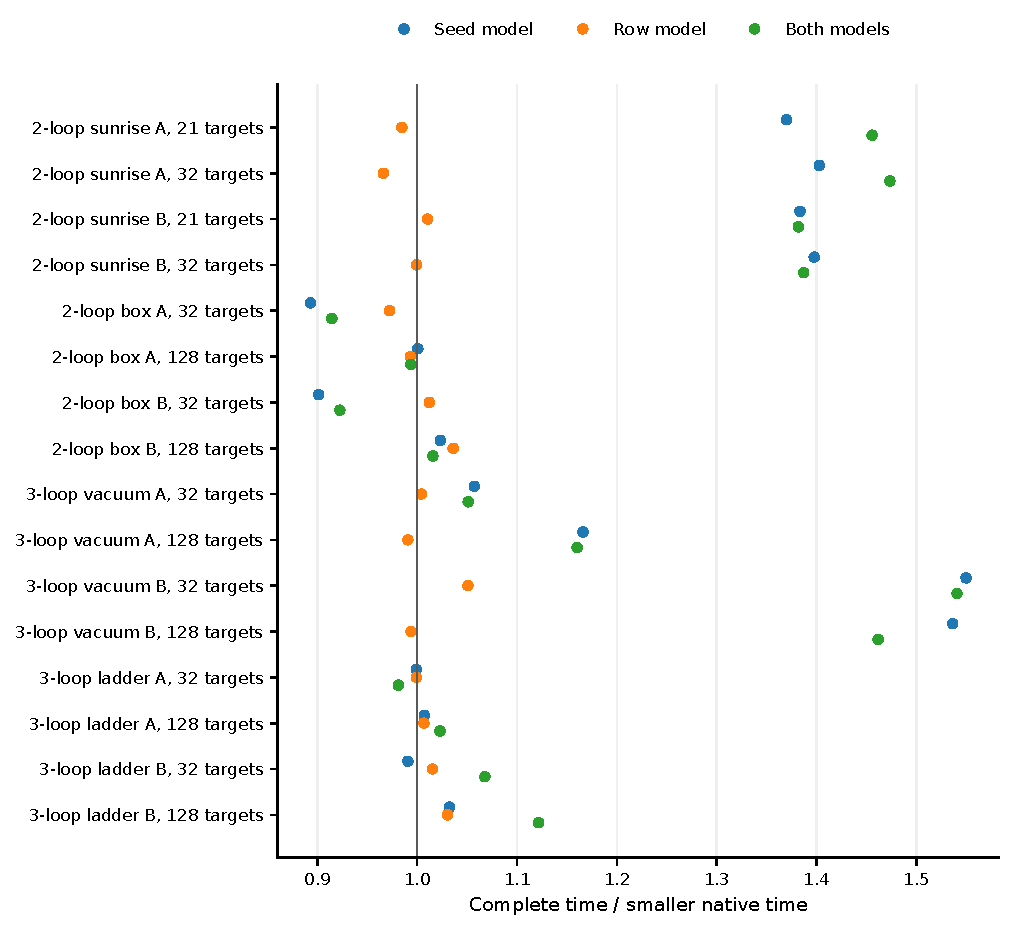
\includegraphics[width=\linewidth]{figures/integrated_runtime_times.pdf}
\caption{Median complete time for the frozen seed, row and combined policies,
divided by the smaller native control's median time on the same target batch.
Every point uses five repeated workflows with fixed physical input and master
basis. Values below one indicate lower complete time. The preceding text
states the timing boundary and profile-weighted intervals.}
\label{fig:integrated-runtime-times}
\end{figure}

\subsection{Elimination work and the contribution of each model}
A lower total runtime can come from seed generation, elimination or shared
execution changes. We therefore also inspect committed forward operations
and compare the combined method directly with the seed-only method.

The row policy relative to native choices gives an operation ratio of 0.985, a forward-stage time ratio of 1.030, and a complete-time ratio of 1.004. The operation count measures the stated coefficient-update proxy. It excludes Fermat's internal polynomial operations, while the two timing measures include the corresponding arithmetic within their stage boundaries.

The combined policy relative to the seed-only method gives an operation ratio of 0.988, a forward-stage time ratio of 1.018, and a complete-time ratio of 1.014. The operation count measures the stated coefficient-update proxy. It excludes Fermat's internal polynomial operations, while the two timing measures include the corresponding arithmetic within their stage boundaries.

The seed model's complete-time ratio to deterministic coverage is 0.978, with interval $[0.872,1.071]$. The row model's ratio to the deterministic cancellation rule is 0.985, with interval $[0.975,0.996]$. Both deterministic controls receive the same feature and runtime optimizations.

Starting from the smaller native region gives a complete-time ratio of 0.502 to the conservative native region. The combined model gives a ratio of 0.585 to that conservative control. The former comparison changes the initial native region without a learned decision. It therefore identifies a shared source of improvement that must be separated from the models' contributions.

\begin{figure}[htbp]
\centering
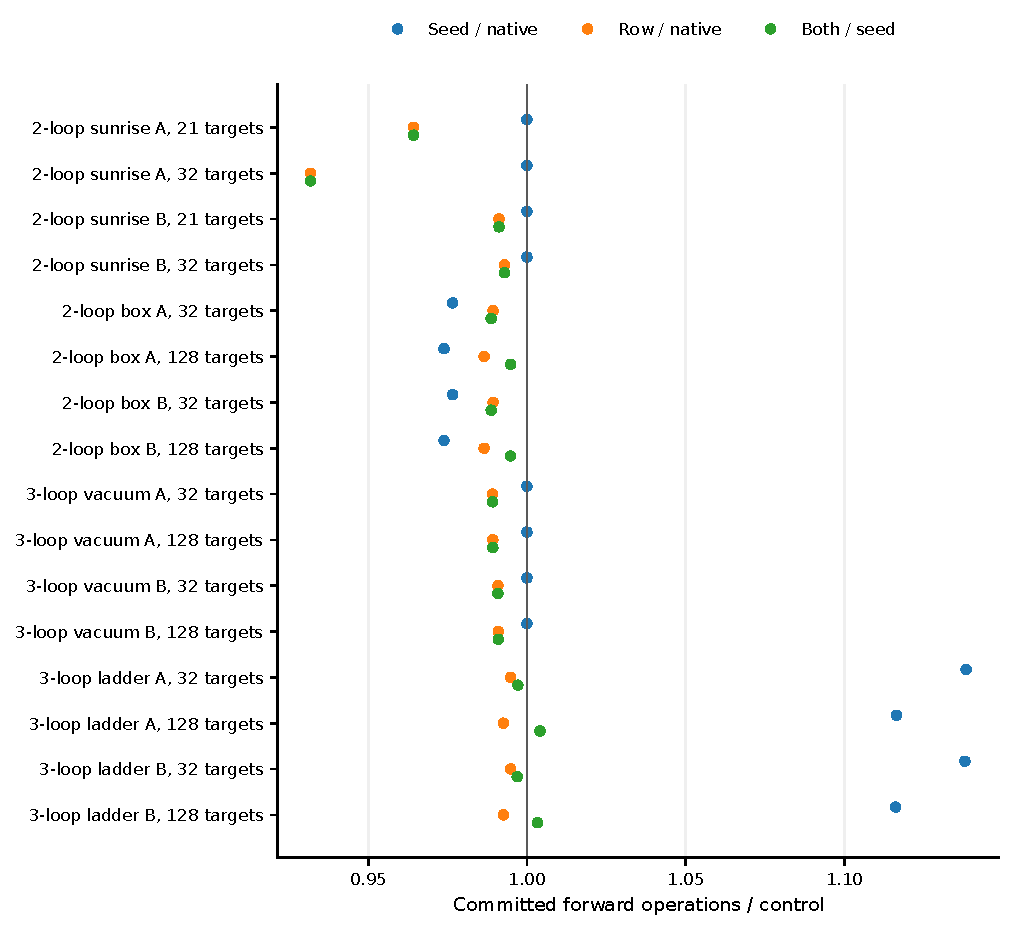
\includegraphics[width=\linewidth]{figures/integrated_runtime_operations.pdf}
\caption{Committed forward coefficient-operation ratios for the seed model
against native choices, the row model against native choices, and the
combined policy against seed selection alone. The last comparison isolates
the additional row policy within the selected seed workflow. These counts
describe the recorded update proxy and do not count internal polynomial work.}
\label{fig:integrated-runtime-operations}
\end{figure}

\subsection{Interpretation of the initial comparison}
The integrated entry point applies the settings fixed from validation.
It can run either model separately, run both models, or select the
validation-recommended method from the topology and target powers.
Automatic selection requires at least a two-percent validation improvement
over the smaller native control; otherwise it retains that control.
Unknown input classes also retain native execution. This rule avoids
paying for models on inputs where development did not support their use.
The reserved ablations above evaluate the fixed choices; reserved timings
do not change their weights or the deployment rule.

The basis check and exact coefficient comparison remain active under every
mode. Incomplete seed sets expand through the fixed fallback, and a
coefficient disagreement in the admitted basis stops the workflow.
The test uses exact rational functions of $d$ at fixed rational masses and
kinematics, with the master basis supplied in advance. Its measured times
exclude discovering and certifying a new generic symbolic basis.

The new row policies learn from complete native trajectories and act inside
Kira's changing matrix. Their allowed action is the source equation among
rows with the same leading integral. They do not choose arbitrary columns,
sectors or all mathematically possible reductions. The finite policy search,
limited physical profiles and descriptive intervals bound the conclusion:
the report establishes the measured changes on the stated inputs, while
a general gain for both models and a globally fastest reduction require
evidence beyond these comparisons.
